%\documentclass{article}
\documentclass[border=5pt]{standalone}
\usepackage{tikz}
\usepackage{bm}
\usetikzlibrary{decorations.markings,decorations.pathreplacing,calc}

\tikzset{help lines/.style={very thin,color=gray!50}} % modify the help lines style
\tikzset{->-/.style={decoration={
  markings,
  mark=at position .5 with {\arrow{>}}},postaction={decorate}}}

\newcommand{\vecbf}[1]{\bm{#1}}
\begin{document}

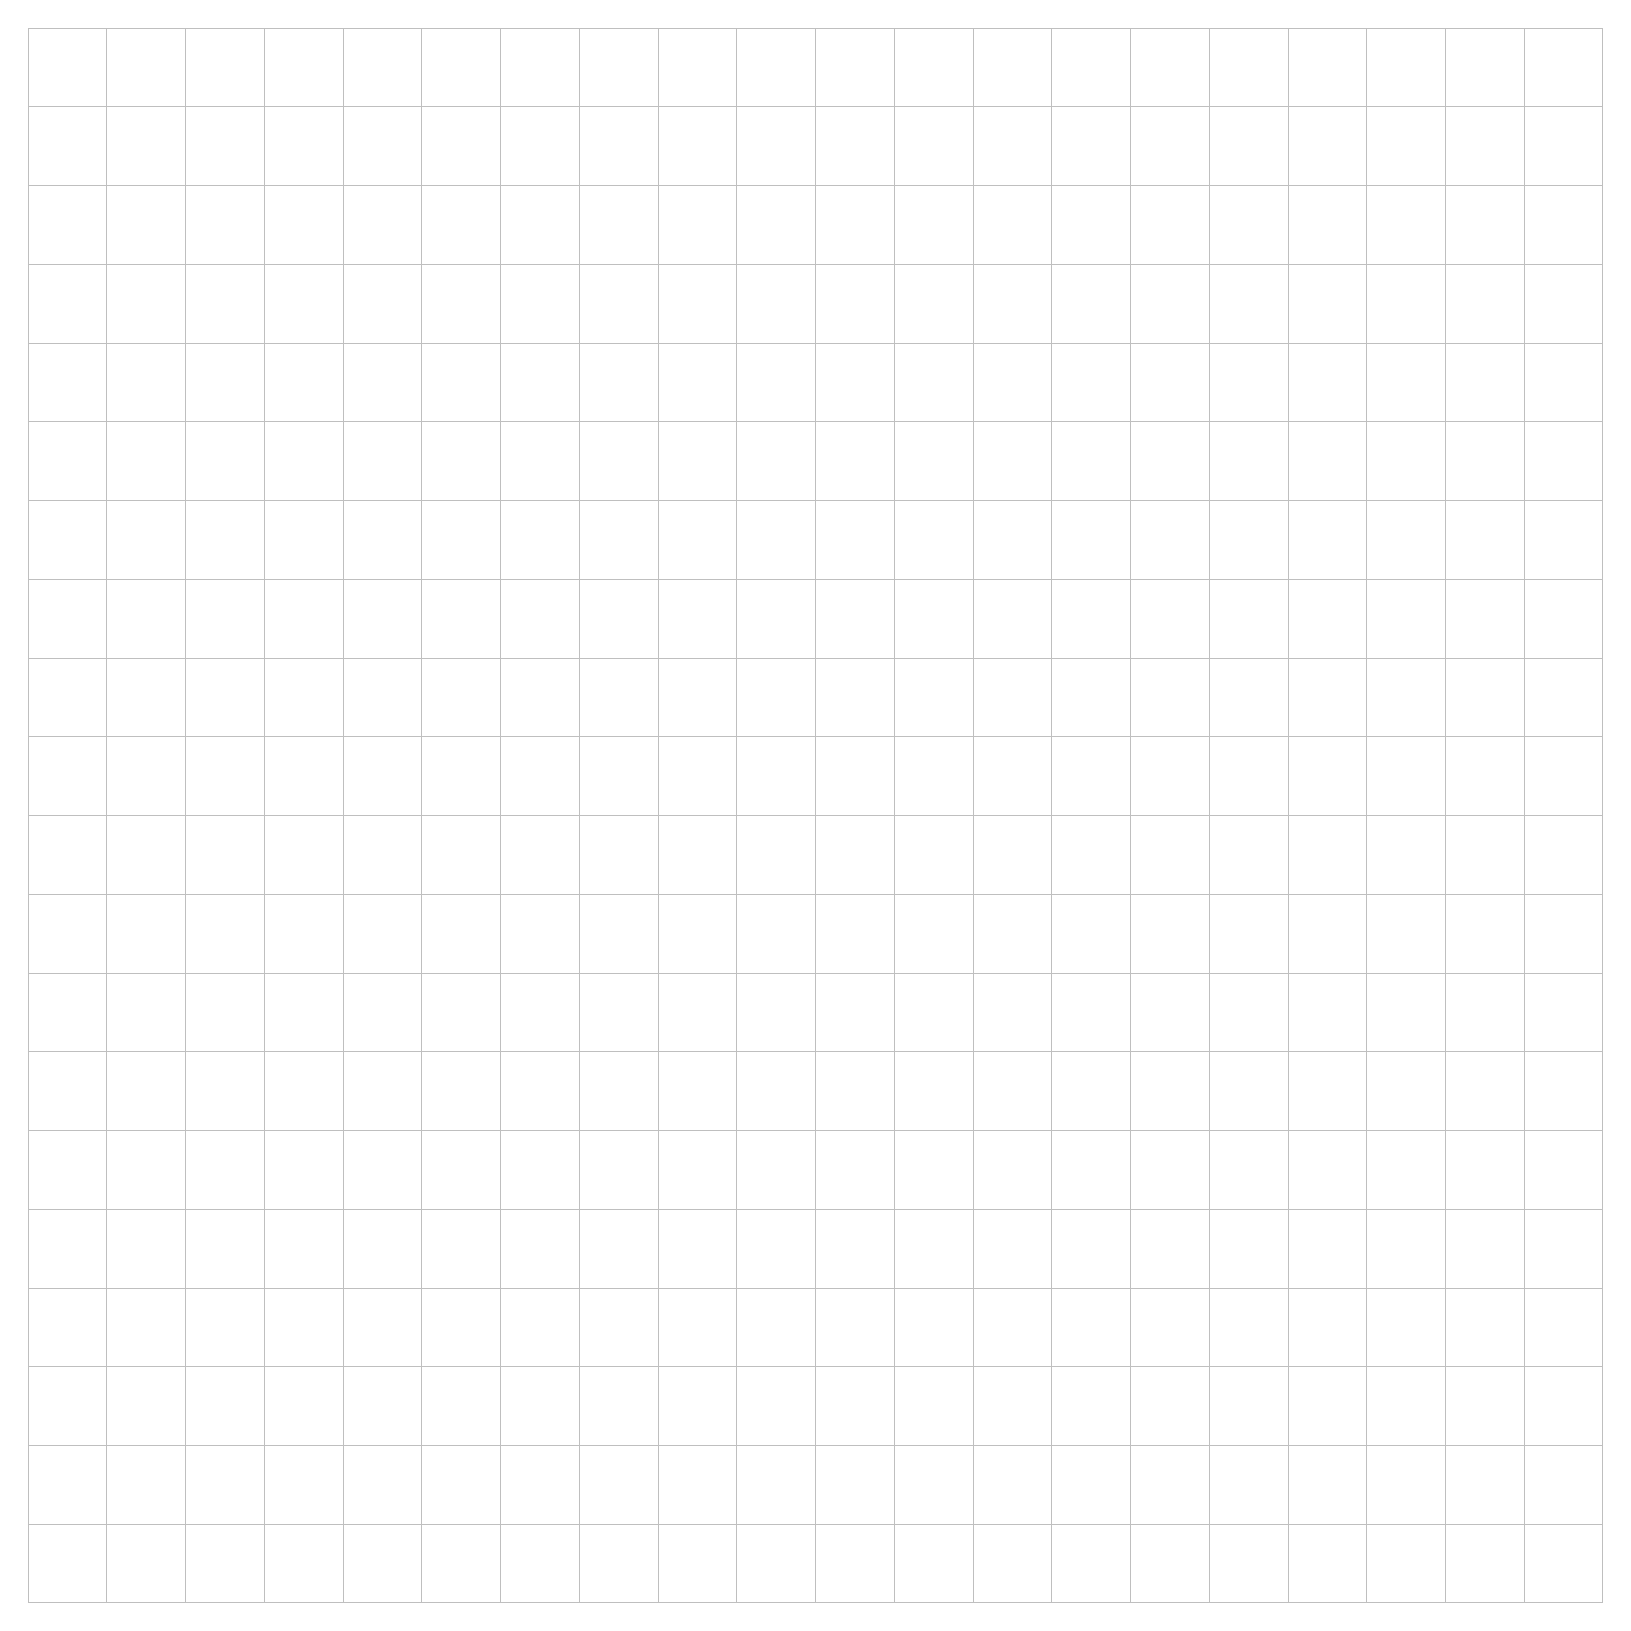
\begin{tikzpicture}[scale=1]
	\draw[help lines] (-10,-10) grid (10,10); %grid
	% \coordinate [label=below:\textcolor{black}{\LARGE \(\vecbf{v}_1\)}] (v1) at (1,-5);
	% \coordinate [label=right:\textcolor{black}{\LARGE  \(\vecbf{v}_2\)}] (v2) at (8,0);
	% \coordinate [label=above:\textcolor{black}{\LARGE  \(\vecbf{v}_3\)}] (v3) at (-1,7);

	% \coordinate (v4) at (-8,3);

	% \coordinate (a_center) at (3,0);
	% \coordinate (b_center) 
	% \draw [ultra thick,black] (v1) --  (v2) -- (v3)  -- (v1);
	% \draw [ultra thick,black] (v1) -- (v4) -- (v3);	
	
\end{tikzpicture}
\end{document}
